\documentclass{article}
\usepackage[utf8]{inputenc}
\usepackage{amsmath}
\usepackage{algorithm}
\usepackage{algpseudocode}
\usepackage{graphicx}  % Para manejar las imágenes
\usepackage{subcaption}  % Para manejar subfiguras
\usepackage{float}  % Opcional para controlar la posición de las figuras


\title{Pr\'actica 1: Complejidad Computacional}
\author{Erick Jes\'us R\'ios Gonz\'alez}
\date{\today}

\begin{document}

\maketitle
\section{Problema del Producto de Subconjuntos}
\subsection{Pseodocódigo}
\begin{algorithm}
\caption{SubsetProductProblem}
\begin{algorithmic}[1]
\Function{generate\_subset}{A: List of Integers} $\to$ List of Integers
    \State Initialize empty list $subset$
    \For{each element $elem$ in $A$}
        \State Generate randomly 0 or 1
        \If{random value is 1}
            \State Add $elem$ to $subset$
        \EndIf
    \EndFor
    \State \Return $subset$
\EndFunction
\\
\Function{verify\_subset}{subset: List of Integers, t: Integer} $\to$ Boolean
    \State Initialize $product = 1$
    \For{each element $elem$ in $subset$}
        \State $product \gets product \times elem$
        \If{$product > t$}
            \State \Return No
        \EndIf
    \EndFor
    \State \Return Yes
\EndFunction
\\
\Function{subset\_product\_decision}{A: List of Integers, t: Integer} $\to$ (Boolean, List of Integers)
    \State $subset \gets$ \Call{generate\_subset}{$A$}
    \State $is\_valid \gets$ \Call{verify\_subset}{$subset, t$}
    \State \Return $(is\_valid, subset)$
\EndFunction
\end{algorithmic}
\end{algorithm}
\subsection{Correctitud}

La función \texttt{generate\_subset} recorre todos los elementos del conjunto $A$ y, para cada elemento, decide aleatoriamente (con probabilidad 50\%) si incluirlo en el subconjunto. Como cada elemento es independiente y el proceso es no determinista, cualquier subconjunto posible de $A$ puede ser generado.
Esto garantiza que el subconjunto generado es un subconjunto válido de $A$, ya que solo puede contener elementos de $A$ y no repite elementos.
La función \texttt{verify\_subset} recibe un subconjunto y calcula el producto de sus elementos. A medida que se va calculando el producto, se verifica si este excede el valor $t$. Si en algún momento el producto excede $t$, se retorna "No" (False). Si el producto es menor o igual a $t$ para todos los elementos, se retorna "Sí" (True).
Esto garantiza que la verificación se realiza correctamente, ya que la multiplicación de elementos y la comparación con $t$ se hace en cada paso, deteniéndose en el momento en que el producto excede $t$.
\subsection{Análisis de Complejidad}

La complejidad del algoritmo es polinomial porque la función generar el subconjunto 
de forma aleatoria es una primitiva, es $O(n)$. Pues no estamos generando
todos los subconjuntos posibles, sino que estamos generando un subconjunto arbitrario.
La función de verificar el producto de los elementos del subconjunto es $O(n)$ también, puesto que
recorremos el subconjunto y multiplicamos los elementos, si el producto excede el valor $t$, 
entonces retornamos No, en caso contrario, retornamos Sí. 
Finalmente la implementación es correcta porque el algoritmo genera un subconjunto de forma aleatoria
y verifica si el producto de los elementos del subconjunto es menor o igual a $t$ en tiempo polinomial.
\subsection{Ejecución del Algoritmo}
\begin{figure}[H]  % 'H' asegura que la figura esté justo aquí (si usas float)
    \centering
    \begin{subfigure}{0.7\textwidth}
        \centering
        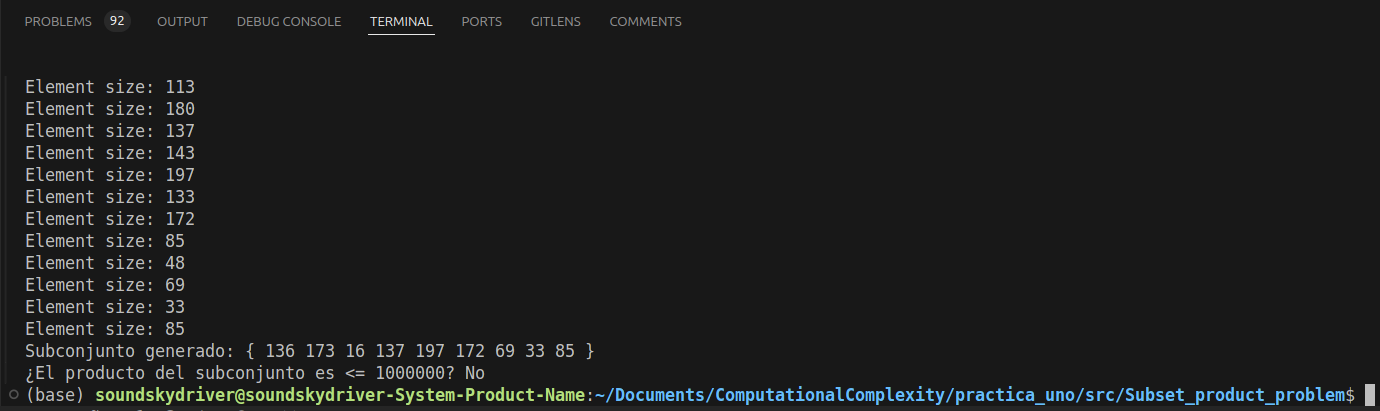
\includegraphics[width=\textwidth]{../images/Screenshot from 2024-09-19 23-21-09.png}
        \caption{Subfigura 1}
        \label{fig:subfig1}
    \end{subfigure}
    \hfill
    \begin{subfigure}{0.7\textwidth}
        \centering
        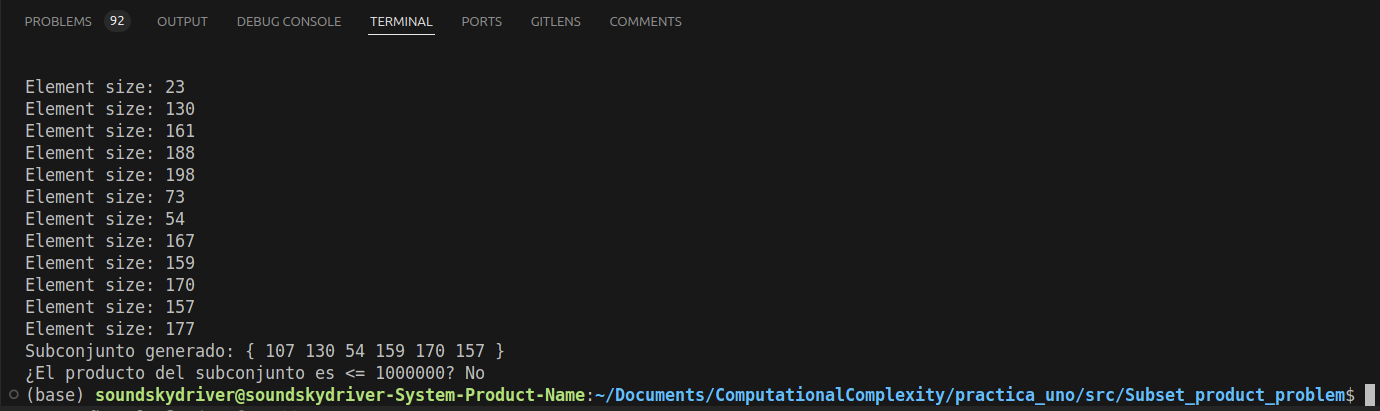
\includegraphics[width=\textwidth]{../images/Screenshot from 2024-09-19 23-21-12.png}
        \caption{Subfigura 2}
        \label{fig:subfig2}
    \end{subfigure}
    \hfill
    \begin{subfigure}{0.7\textwidth}
        \centering
        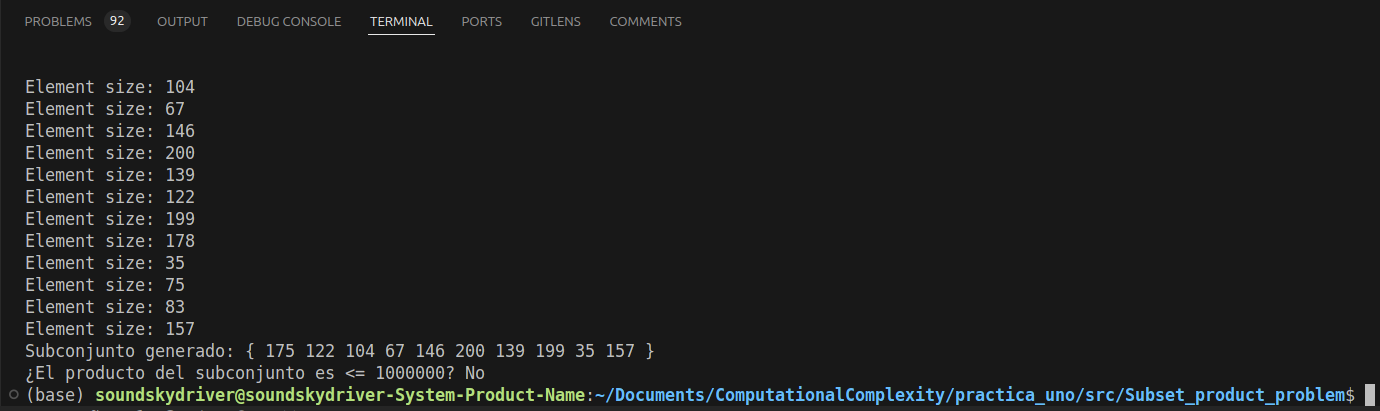
\includegraphics[width=\textwidth]{../images/Screenshot from 2024-09-19 23-21-17.png}
        \caption{Subfigura 3}
        \label{fig:subfig3}
    \end{subfigure}

    \vspace{10pt}  % Espacio vertical entre las filas de subfiguras

    \begin{subfigure}{0.7\textwidth}
        \centering
        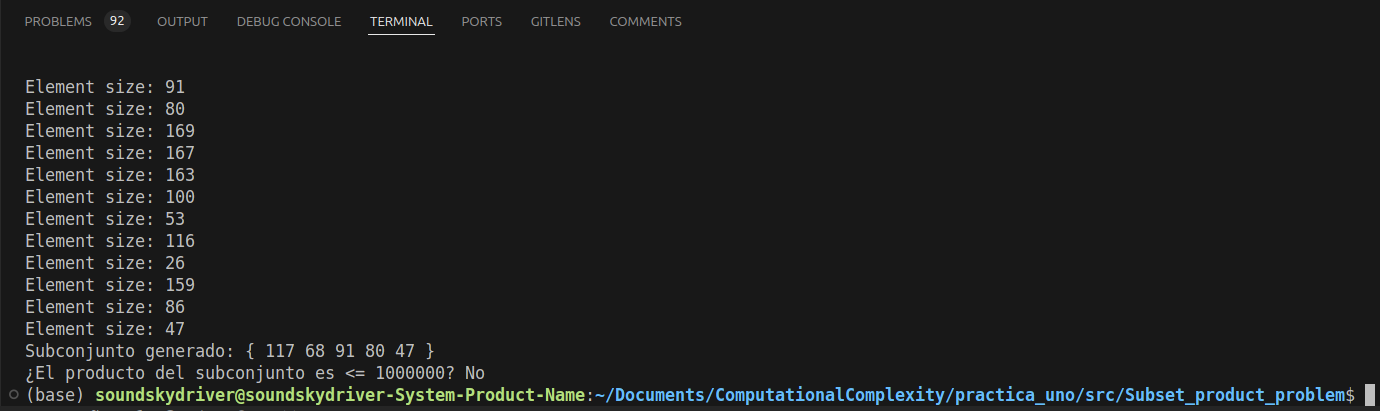
\includegraphics[width=\textwidth]{../images/Screenshot from 2024-09-19 23-21-22.png}
        \caption{Subfigura 4}
        \label{fig:subfig4}
    \end{subfigure}
    \hfill
    \begin{subfigure}{0.7\textwidth}
        \centering
        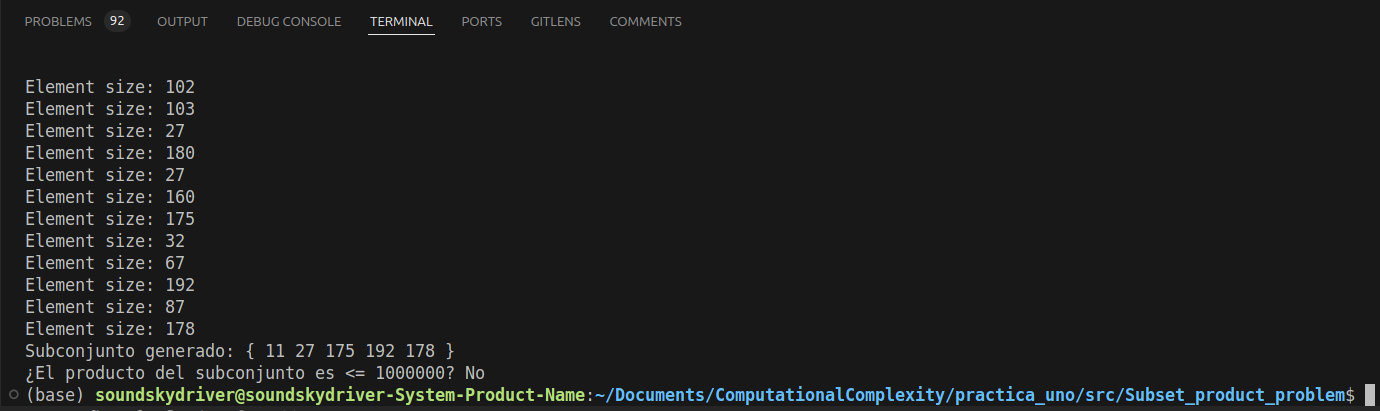
\includegraphics[width=\textwidth]{../images/Screenshot from 2024-09-19 23-21-26.png}
        \caption{Subfigura 5}
        \label{fig:subfig5}
    \end{subfigure}

    \caption{Cinco ejecuciones del algoritmo desde terminal}
    \label{fig:all_subfigures}
\end{figure}


\section{Problema de la Mochila}
\section{Pseodocódigo}
\begin{algorithm}
    \caption{Knapsack Problem Solver}
    \begin{algorithmic}[1]
    
    \Function{generate\_subset}{Item: List of [item\_weight, value]} $\to$ List of Integers
        \State Initialize empty list $subset$
        \For{each element $elem$ in Item}
            \State Generate randomly 0 or 1
            \If{random value is 1}
                \State Add $elem$ to $subset$
            \EndIf
        \EndFor
        \State \Return $subset$
    \EndFunction

    \Function{verify\_subset}{subset: List of Integers, max\_capacity: Integer} $\to$ {Boolean, Integer}
        \State Initialize $total\_value \gets 0$
        \For{each element $elem$ in subset}
            \State $total\_weight \gets total\_weight + elem.weight$
            \State $total\_value \gets total\_value + elem.value$
            \If{$total\_weight >= max\_capacity$}
                \State \Return (Yes, $total\_value$)
            \Else
                \State \Return (No,0)
            \EndIf-else
        \EndFor
    \EndFunction

    \Function {knapsack\_solver}{Item: List of [item\_weight, value], max\_capacity: Integer} $\to$ (Boolean, List of Integers)
        \State $subset \gets$ \Call{generate\_subset}{Item}
        \State $(is\_valid, total\_value) \gets$ \Call{verify\_subset}{subset, max\_capacity}
        \State \Return $(is\_valid, total\_value)$
    \EndFunction
    \end{algorithmic}
\end{algorithm}
\subsection{Correctitud}
La función \texttt{generate\_subset} recorre todos los elementos del conjunto $Item$ y, para cada elemento, decide aleatoriamente (con probabilidad 50\%) 
si incluirlo en el subconjunto. Como cada elemento es independiente y el proceso es no determinista, cualquier subconjunto posible de $Item$ puede ser generado.
Esto garantiza que el subconjunto generado es un subconjunto válido de $Item$, ya que solo puede contener elementos de $Item$ y no repite elementos.
La función \texttt{verify\_subset} recibe un subconjunto y calcula el peso total de sus elementos, así como la ganancia total. A medida que se va calculando el peso
total, se verifica si este excede el valor $max\_capacity$. Si en algún momento el producto excede $max\_capacity$, se retorna "No" (False). Si el producto es menor o igual a $\max_capacity$ para todos los elementos, se retorna "Sí" (True).
Esto garantiza que la verificación se realiza correctamente, ya que la suma de los pesos y la comparación con $max\_capacity$ se hace en cada paso, deteniéndose en el momento en que el $total\_weight$ excede $max\_capacity$.

\textbf{Nota}: Para la implementación el programa nos pide encontrar el subconjunto que maximiza la ganancia, por lo que creo un ciclo for con un número de iteraciones definidas desde el inicio, en este caso 1000 iteraciones.
Esto sigue siendo correcto, pues durante un numero finito de iteraciones, se generan subconjuntos aleatorios y se verifica si el peso total excede la capacidad máxima. De esta forma obtenemos un 
maximo local que maximiza la ganancia.
\subsection{Análisis de Complejidad}
La complejidad del algoritmo es polinomial porque la función generar el subconjunto 
de forma aleatoria es una primitiva, es $O(n)$. Pues no estamos generando
todos los subconjuntos posibles, sino que estamos generando un subconjunto arbitrario.
La función de verificar el producto de los elementos del subconjunto es $O(n)$ también, puesto que
recorremos el subconjunto y sumamos los pesos de los elementos, si el peso total excede el valor $max\_capacity$, 
entonces retornamos No, en caso contrario, retornamos Sí. 
Finalmente la implementación es correcta porque el algoritmo genera un subconjunto de forma aleatoria
y verifica si el producto de los elementos del subconjunto es menor o igual a $max\_capacity$ en tiempo polinomial.

\textbf{Nota}: La implementación utilizando un número finito de iteraciones sigue siendo polinomial, pero el algoritmo no garantiza que el subconjunto generado sea el óptimo, sino que es un subconjunto que maximiza la ganancia en un número finito de iteraciones.

\subsection{Ejecución del Algoritmo}

\begin{figure}[H]  % 'H' asegura que la figura esté justo aquí (si usas float)
    \centering
    \begin{subfigure}{0.7\textwidth}
        \centering
        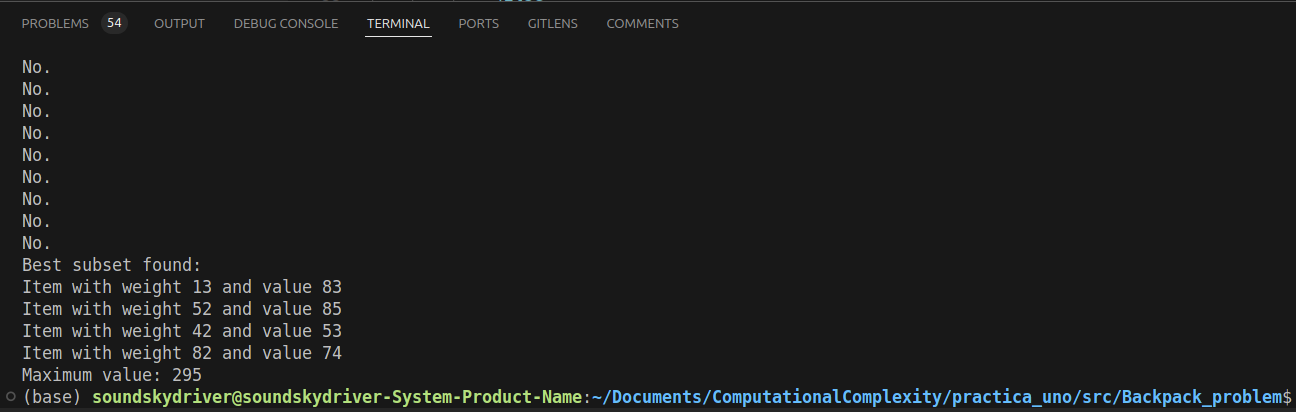
\includegraphics[width=\textwidth]{../images/Screenshot from 2024-09-19 23-04-13.png}
        \caption{Subfigura 1}
        \label{fig:subfig1}
    \end{subfigure}
    \hfill
    \begin{subfigure}{0.7\textwidth}
        \centering
        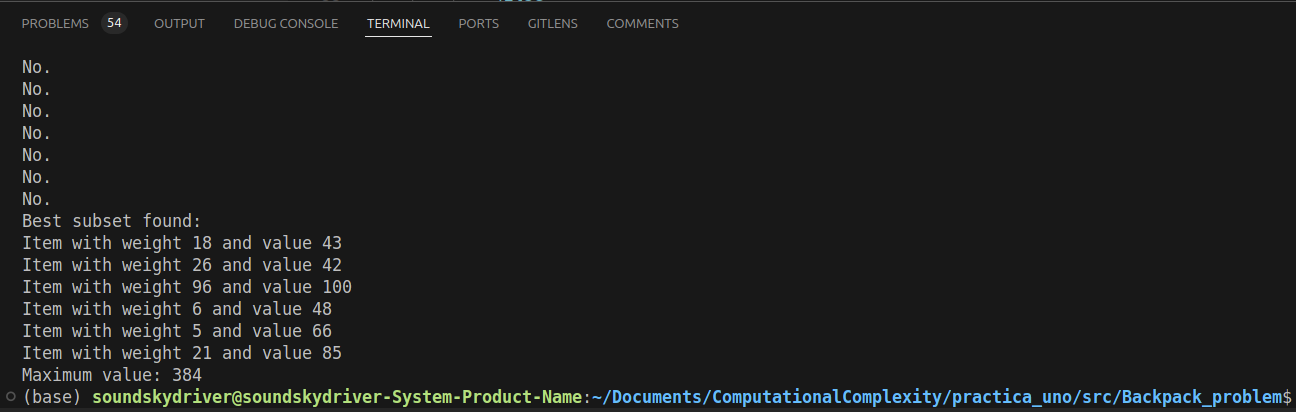
\includegraphics[width=\textwidth]{../images/Screenshot from 2024-09-19 23-03-51.png}
        \caption{Subfigura 2}
        \label{fig:subfig2}
    \end{subfigure}
    \hfill
    \begin{subfigure}{0.7\textwidth}
        \centering
        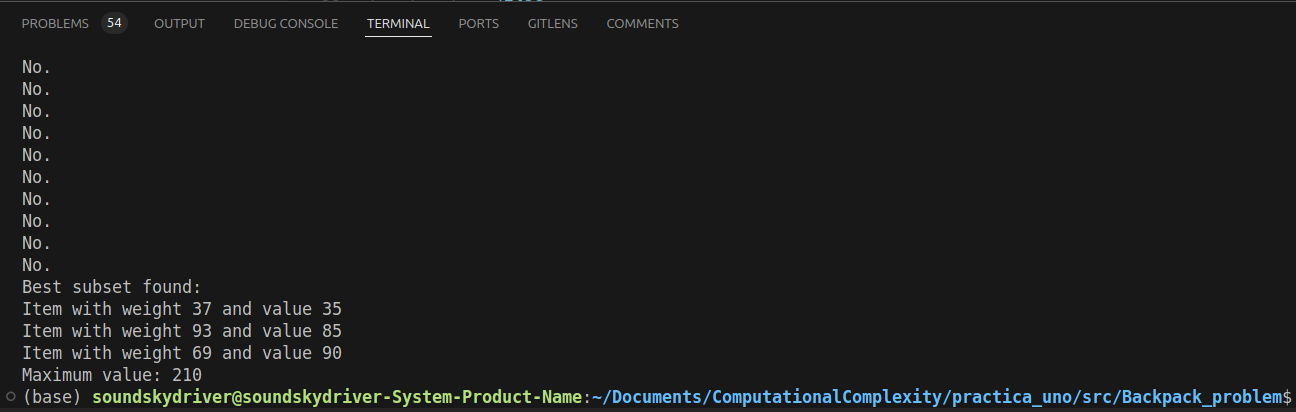
\includegraphics[width=\textwidth]{../images/Screenshot from 2024-09-19 23-03-59.png}
        \caption{Subfigura 3}
        \label{fig:subfig3}
    \end{subfigure}

    \vspace{10pt}  % Espacio vertical entre las filas de subfiguras

    \begin{subfigure}{0.7\textwidth}
        \centering
        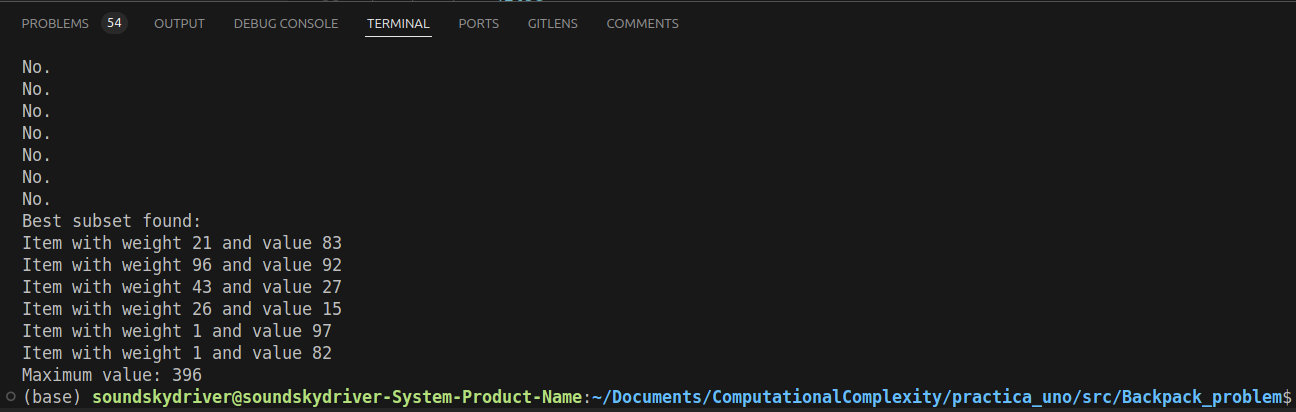
\includegraphics[width=\textwidth]{../images/Screenshot from 2024-09-19 23-04-05.png}
        \caption{Subfigura 4}
        \label{fig:subfig4}
    \end{subfigure}
    \hfill
    \begin{subfigure}{0.7\textwidth}
        \centering
        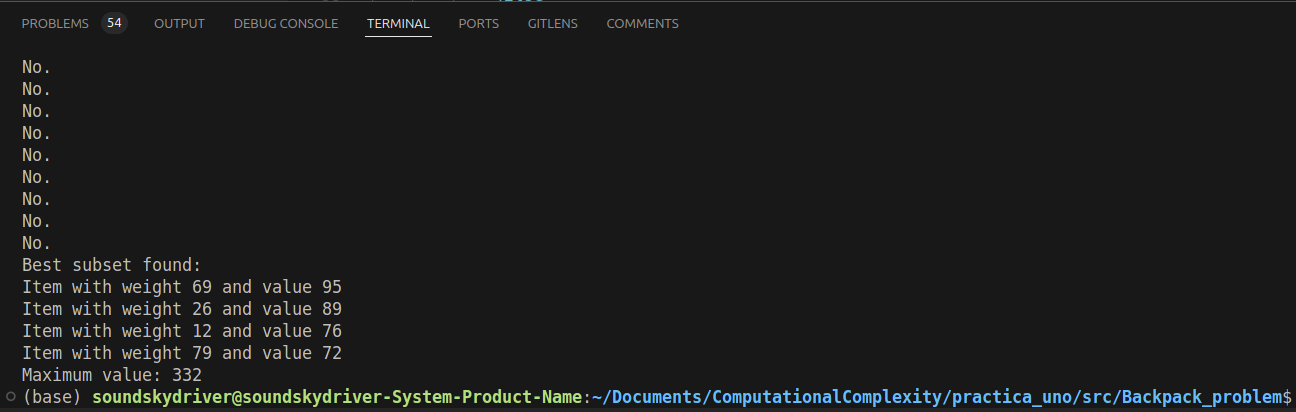
\includegraphics[width=\textwidth]{../images/Screenshot from 2024-09-19 23-04-09.png}
        \caption{Subfigura 5}
        \label{fig:subfig5}
    \end{subfigure}

    \caption{Cinco ejecuciones del algoritmo desde terminal}
    \label{fig:all_subfigures}
\end{figure}
\end{document}
